\documentclass[a4paper,12pt]{article}
\usepackage{geometry}
\usepackage{hyperref}
\usepackage{amsmath}
\usepackage[utf8x]{inputenc}
\usepackage{libertine}
\usepackage{dsfont}
\usepackage{graphicx}

\hypersetup{
    colorlinks=true,
    linkcolor=blue,
    filecolor=magenta,      
    urlcolor=cyan,
}

\geometry{margin=1in}

\begin{document}
\title{Empirical IO Homework}
\author{Andrei Zaloilo, Wenxuan Xu}
\maketitle

\section{Estimation of the Model}

\subsection{Random Coefficient Logit}

We estimate the standard random coefficeint logit model for the French automobile market, placing a single random coefficient on the price. Specifically, we assume that utility satisfies the following linear specification:
\begin{equation}
    u_{ijt} = X_{jt}*\beta + \alpha_{i} * p_{jt} + \zeta_{jt} + \epsilon_{ijt}
\end{equation}
where $X_{jt}$ are car characteristics for product $j$ in time $t$, i.e.\ cylinder, weight, horsepower and fuel cost and a constant, $p_{jt}$ is the corresponding price, $\zeta_{jt}$ is a product-time specific unobserved heterogeneity, while $\epsilon_{ijt}$ is an individual-product-time specific unobserved heterogeneity that is $i.i.d.$ extreme value type 1 distributed. 

Here, $\beta$ is a common preference among all consumers regarding product characteristics, while $\alpha_i = \alpha + \sigma v_i$ are individual specific sensitivities to price, which we will assume to be decomposable to a population wide parameter $\alpha$ and normally distributed preference $\sigma v_i \sim N(0, \sigma^2)$.

In (i) of Table \ref{m1}, we find the estimated $\sigma$ to be 0.675 and the estimated coefficients to be positive for weight and horsepower, and negative for cylinder, fuel cost and price. These signs are generally expected with consumers prefering heavier or larger cars, more horsepower, less fuel cost, a cheaper price, and a smaller cylinder conditional on horsepower, corresponding to possibly better quality engines .

Normalizing by the coefficient on price, this means that an average consumer is willing to pay \texteuro 205 to decrease a car's cylinder capacity by $1000 cm^3$, to pay \texteuro 1109 to increase the weight by $1000 kg$, to pay \texteuro 1152 to increase the horsepower by 1 unit, and \texteuro 2147 to decrease its fuel cost by 1 \texteuro / 100km.

\subsection{Year and Brand Fixed effect}

We modify (1) with year and brand fixed effects:
\begin{equation}
    u_{ijt} = X_{jt}*\beta + \alpha_{i} * p_{jt} + a_j + a_t + \zeta_{jt} + \epsilon_{ijt}
\end{equation}
where $a_j$ and $a_t$ are brand and year fixed effects respectively. We present the results as (ii) in Table \ref{m1}. We can see that the coefficients estimated retain their signs. Having smaller cylinders is much more important for consumers than without fixed effects. While weight and price are also more important factors that were previously masked by not including brand and year fixed effects. 

\subsection{Differentiated IV}
Instead of just using the product characteristics IVs in the data, we construct local differentiation IVs by using:
\begin{align*}
    \sum_{j'} |d^l_{jt,j'}| \mathds{1}(|d^l_{jt,j'}| < \sigma_{l,t}) \quad , \sum_{j'} |d^{\hat{p}}_{jt,j'}|\mathds{1}(|d^{\hat{p}}_{jt,j'}|<\sigma_{p,t})
\end{align*}
We use these instruments in addition to the original BLP instruments to estimate (iii) in Table \ref{m1}. By using the diffentiated IVs, we see a significant fall in the importance of price estimated in the utility function, at the same time implying less consumer heterogeneity.

\begin{table}[h!]
    \centering
    \caption{BLP Demand Estimates}
    \begin{tabular}{rrrr} 
    \hline\hline
                              & (i)     & (ii)   & (iii)  \\ 
    \hline
    Cylinder                  & -0.037  & -0.215 & -0.184 \\
    Weight                    & 0.199   & 0.363  & 0.306 \\
    Horsepower                & 0.207   & 0.190  & 0.186  \\
    Fuel                      & -0.385  & -0.338 & -0.337  \\
    Price                     & --1.794 & -5.035 & -3.781\\
    $\sigma$ & 0.675   & 2.239  &    1.618    \\ 
    \hline
    FE                        & No      & Yes    & Yes    \\
    N                         & 5028    & 5028   & 5028   \\
    \hline\hline
    \end{tabular}
    \label{m1}
\end{table}

\newpage    
\section{Counterfactual Simulation}

In this section, we take simulate counterfactuals that occur in the year 2008, using the 2008 estimated marginal costs and set of products.

\subsection{Mergers}

We simulate a merger between Volkswagen and BMW in 2008. Comparing the average price, average markup, total industry profits, average consumer surplus and profits of the merging parties in Table \ref{m2}, we see that the merger though beneficial for the merging parties and the industry as a whole, increasing profits from \texteuro 7.17 billion to \texteuro 7.22 billion, a total of 6.3\%, but weighs negatively on the average consumer surplus, dropping it by 0.4\% or \texteuro 3 per consumer. The result is an increase in average price, an increase in average markup, greater profits for both companies' original products, and a more profitable industry as a whole.

\begin{table}[h!]
    \centering
    \caption{Counterfactual Merger between Volkswagen and BMW (in \texteuro 10,000)}
    \begin{tabular}{lll} 
    \hline\hline
                          & Pre-merger & Post-merger  \\ 
    \hline
    Average Price         & 3.1062     & 3.1300       \\
    Average Cost          & 2.2895     & 2.2895       \\
    Average Markup        & 0.3507     & 0.3585       \\
    Total Industry Profit & 717240     & 721902       \\
    Average CS            & 0.3330     & 0.3317       \\
    Average Volks Price   & 3.1597     & 3.2145       \\
    Average BMW Price     & 4.7861     & 4.9550       \\
    Average Volks Markup  & 0.3541     & 0.3734       \\
    Average BMW Markup    & 0.3765     & 0.4255       \\
    Total Volks Profits   & 89916      & 90304        \\
    Total BMW Profits     & 36348      & 36373        \\
    \hline\hline
    \end{tabular}
    \label{m2} 
 \end{table}
\subsection{Efficiency Gains}

In order to see what level of efficiency gains must be necessary for such a merger to be net neutral to consumer surplus, we simulate a percentage reduction in the marginal cost of all products owned by the merging parties in 2008. As shown in Figure \ref{efficiency}, average consumer surplus is strictly increasing in efficiency gains and very close to linear. The result suggests that a percentage reduction in marginal cost of around 1.75\% for all products of the merging parties is necessary such that there is no fall in average consumer surplus after the merger.

\begin{figure}[h!]
    \centering
    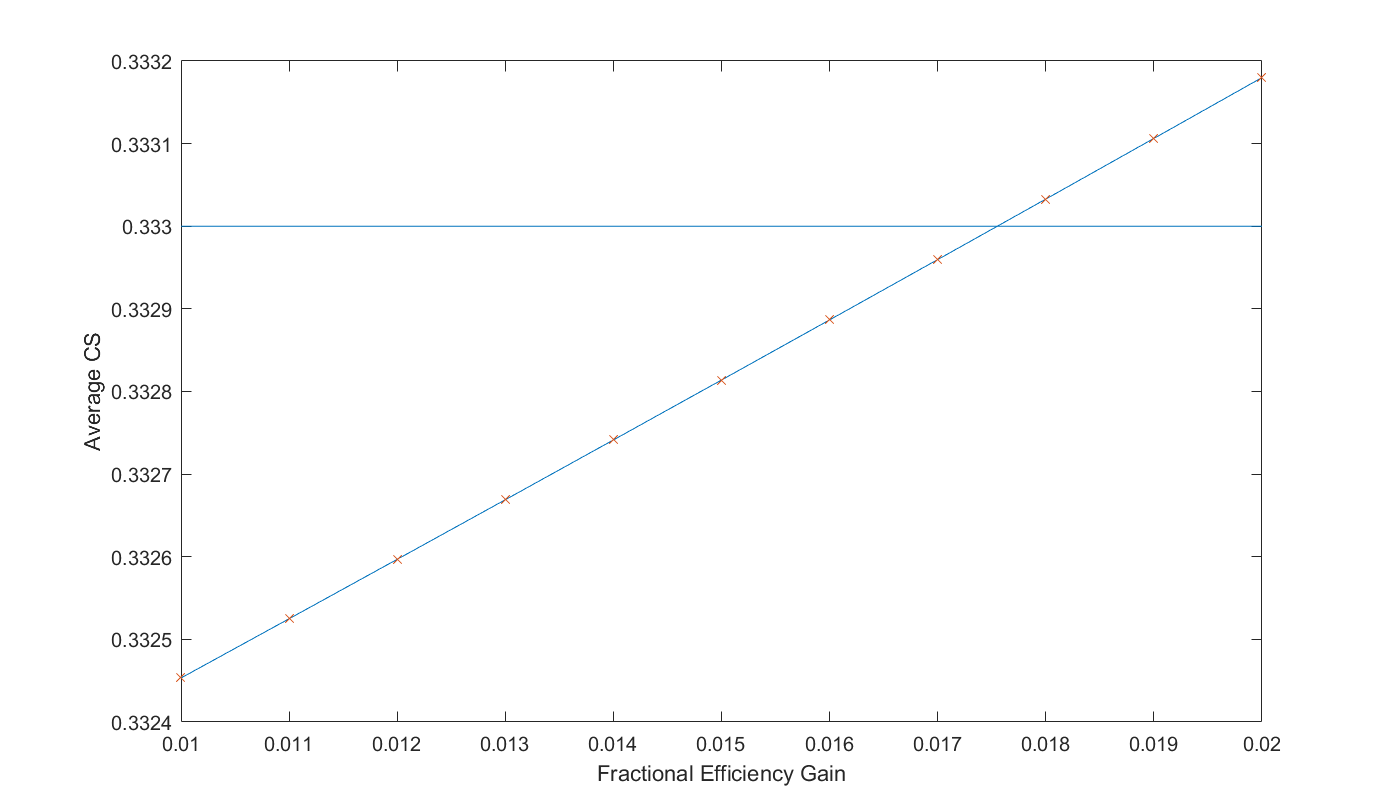
\includegraphics[scale=0.4]{efficiency.png}
    \caption{Plot of Average CS against Fractional Efficiency Gain for Merging Parties}
    \label{efficiency}
\end{figure}

\section{Cross Participation}

\subsection{One-sided Ownership}

We consider the effect on the market equilibrium when Renault purchases 30\% shares of PSA. When this happens, we assume that Renault now internalizes 30\% of the impact of its pricing decisions on PSA's market shares, but not the other way around. In the final calculation of profits, we add 30\% of PSA's profits to Renault's profits to obtain the adjusted profits.

The results as shown in Table \ref{m3} (R buys P). We see that average price increases by 0.7\% and markup increases by 4.9\%. Additionally, the (unadjusted) profits of Renault decrease and that of PSA increases in line with our intuition on the internalization effect. The total industry profit increases, and the average consumer surplus falls. This is due to the weakening of competitive pressure that results from Renault internalizing part of PSA's profits in its pricing decisions.

\subsection{Two-sided Ownership}

If PSA buys 30\% of Renault, we again have a symmetric ownership matrix. We rationalize this approach as an approach that takes the firms' position rather than the shareholders' position in production decisions. Firm's own equity in each other, and make production decisions maximizing 100\% of its own production profits and its 30\% pure equity holdings. This contrasts with the shareholders' position which will maximize a 70-30 split between the production profits of its majority-minority ownership firms.

This is presented as P buys R (Mutual) in Table \ref{m3}. This means that PSA is willing to pay up to \texteuro 481.4 million for 30\% ownership of Renault, when Renault already owns 30\% of PSA.

On the other hand, if Renault had not already bought PSA shares, PSA needs to factor in only its own changes in pricing decisions when it purchases Renault shares, which is compensated by Renault's unfettered pricing decisions. In all, this means that there is an increase in the willingness to pay to \texteuro 481.7 million, as compared to the case of mutual cross-ownership.

The consideration here is that if Renault and PSA are good substitutes, they would be better off owning each others' shares and dampening competition. Their merger is however going to be of a greater benefit to the industry than themselves, since their competitors benefit more from the merger raising prices.

\begin{table}[h!]
    \centering
    \caption{Cross Participation Counterfactuals (in \texteuro 10,000)}
    \begin{tabular}{lrrrr}
        \hline \hline


                           & \multicolumn{1}{l}{Baseline} & \multicolumn{1}{l}{R buys P} & \multicolumn{1}{l}{P buys R} & \multicolumn{1}{l}{P buys R (Mutual)}  \\ 
    \hline     Average Price          & 3.1062                       & 3.1085                       & 3.1088                       & 3.1112                                 \\ 
    Average Markup         & 0.3507                       & 0.3524                       & 0.3525                       & 0.3542                                 \\
    Renault Profits        & 159676                       & 159443                       & 161059                       & 160826                                 \\
    PSA Profits            & 226091                       & 228074                       & 225940                       & 227924                                 \\
    Renault Profits (Adj.) & 159676                       & 227865                       & 112741                       & 180956                                 \\
    PSA Profits (Adj.)     & 226091                       & 159652                       & 274258                       & 207795                                 \\
    Total Industry Profits & 717240                       & 721746                       & 721201                       & 725778                                 \\
    Average CS             & 0.33304                      & 0.33168                      & 0.33172                      & 0.33034                                \\
    WTP                    & -         & 68189                        & 48167                        & 48143 \\
    \hline\hline                                
    \end{tabular}
    \label{m3}
\end{table}

\end{document}